\documentclass[12pt]{article}
\usepackage[german]{babel}
\usepackage{amsmath}
\usepackage{amssymb}
\usepackage{stmaryrd}
\usepackage{xcolor}
\usepackage{setspace}
\usepackage[margin=2cm,left=4cm,marginparwidth=3cm]{geometry}
\usepackage{listings}
\usepackage{float}
\usepackage{graphicx}
\usepackage{amsfonts}
\reversemarginpar

\lstset{
language=Python,
numbers=left,
keepspaces=true,
keywordstyle=\color{blue},
morekeywords={assert},
basicstyle=\footnotesize\ttfamily,
numberstyle=\tiny\color{gray},
commentstyle=\color{teal},
stringstyle=\color{purple},
title=\lstname,
captionpos=b,
}
\lstdefinelanguage{none}{
  identifierstyle=
}
\newfloat{code-snip}{htbp}{what_is_this}
\floatname{code-snip}{Quellcodeausschnitt}

% https://tex.stackexchange.com/a/30114
\setstretch{1.241}

\newcommand{\todo}[1]{\textcolor{red}{\mbox{TODO}}\marginpar{\textcolor{red}{#1}}}
\newcommand{\floor}[1]{\lfloor #1 \rfloor}

% https://tex.stackexchange.com/questions/23957/how-to-set-font-to-arial-throughout-the-entire-document
\renewcommand{\rmdefault}{phv} % Arial
\renewcommand{\sfdefault}{phv} % Arial

\title{Mathematische Hintergr\"unde und praktische Anwendung asymmetrischer Kryptographie am Beispiel von RSA und OpenPGP}
\input{pii.tex}

\begin{document}
\maketitle
\thispagestyle{empty}
\newpage
\tableofcontents
\thispagestyle{empty}
\newpage

\section{Einleitung}
% Asymmetrische Kryptographie ist toll. Damit kann man vieles machen (verschl"usseln, unterschreiben). [Bild von Wikipedia] Im "`digitalen Zeitalter"' ist das wichtig. (TLS, IoT). OpenPGP (Phil Zimmermann) ist neben S/MIME das Standardprotokoll f"ur krypto-behandelte E-Mails, hat aber auch z.B. WoT. Ich habe einen Teil davon implementiert.

Traditionell waren Verschl"usselungsverfahren "`symmetrisch"', d.h., dass wie bei einem physischen Schloss
der gleiche Schl"ussel zum Verschlie"sen (Verschl"usseln) und zum Aufschlie"sen (Entschl"usseln) verwendet wird.
Der Ver\-schl"us\-sel\-ungs\-pro\-zess ist im Laufe der Zeit komplizierter geworden
(von der auch im Kopf m"oglichen Caesar-Verschl"usselung bis zur
maschinellen Verschl"usselung der Enigma w"ah\-rend des zweiten Weltkriegs),
jedoch hat es nie bis zuletzt
eine Abweichung vom Konzept eines einzigen Schl"ussels f"ur Ver- und Entschl"usselung gegeben.

Nach Entwicklung der Vorl"aufer des heutigen Internets wurde dann die asymmetrische Kryptographie erfunden.
Hier werden f"ur Ver- und Entschl"usselung separate Schl"ussel verwendet
(wie bei einem Vorh"angeschloss, wenn man das Schlie"sen als "`"offentlichen Schl"ussel"' betrachtet),
sodass Menschen verschl"usselt kom\-mu\-ni\-zie\-ren k"onnen, ohne vorher einen gemeinsamen Schl"ussel auszutauschen.
Neben Verschl"usselung von Nachrichten kann das Konzept asymmetrischer Kryptographie
auch f"ur digitale Unterschriften verwendet werden.

Der erste solche Verschl"usselungsalgorithmus, der auch in der Lage ist, Unterschriften zu erstellen und zu verifizieren, ist RSA\@.
Diesen m"ochte ich in dieser Arbeit n"aher betrachten und auch selbst implementieren.
RSA wird weiterhin in verschl"usselten Verbindungen mit gr"o"seren Seiten
wie etwa \texttt{wikipedia.org}, \\ \texttt{google.com} oder \piibigsite{} verwendet.%
\footnote{Obwohl sowohl Google als auch Wikipedia inzwischen ECC-Schl"ussel verwenden,
sind die Schl"ussel der entsprechenden Root-CAs noch immer RSA-2048 (Stand \today)}

Neben dieser Anwendung in TLS (der Kryptographie-Komponente\footnote{
TLS ist trotz dieser massiven Anwendung im WWW ein separates Protokoll und wird auch z.B. f"ur SMTPS oder FTPS (nicht mit SFTP zu verwechseln, welches "uber SSH l"auft) verwendet}
von HTTPS, dem Protokoll f"ur das WWW) wird RSA auch in OpenPGP,
welches auf dem 1991 von Phil Zimmermann ver"offentlichten PGP basiert und Einsatz bei der Ende-zu-Ende-Verschl"usselung
(d.h., dass nur Sender und Empf"anger den Inhalt lesen k"on\-nen)
von E-Mails findet, zur Verschl"usselung und f"ur Unterschriften verwendet.
W"ah\-rend sich OpenPGP auch mit der Vernetzung von Schl"usseln im Sinne eines sog.\@ "`Web of Trust"' befasst,
habe ich mich bei meiner Teilimplementation haupts"achlich auf die durch RSA m"oglich gemachten
Funktionalit"aten konzentriert\footnote{Wobei nat"urlich Unterschriften "uber Schl"ussel f"ur das WoT wichtig sind, und ich somit diesen Teilaspekt mitimplementiert habe}.

In dieser Facharbeit sollen die mathematischen Grundlagen von RSA beleuchtet und
fachlich korrekt sowie allgemein verst"andlich erkl"art werden,
einige konkrete Hinweise f"ur eine praktische Umsetzung angesprochen werden
sowie am Beispiel der Einbettung von RSA in OpenPGP tats"achliche praktische
Eins"atze asymmetrischer Kryptographie dargestellt werden.
Im Verlauf soll progressive eine Entwicklung von den mathematischen Hintergr"unden
hin zur praktischen Anwendung ersichtlich werden.

\section{Mathe hinter RSA}
%Nachrichten und Schl"ussel sind Zahlen.
%Hier wahrscheinlich sehr viel aus dem RSA-Paper zitieren.

Mathematisch betrachtet man eine Nachricht als eine Zahl und einen
Ver\-schl"us\-sel\-ungs\-al\-go\-rith\-mus als zwei Funktionen.
Eine, im Folgenden $E(m)$, verwandelt unter Zuhilfenahme eines Schl"ussels eine
Nachricht in chiffrierten Text, eine zweite, im Folgenden $D(c)$,
verwandelt unter Zuhilfenahme eines anderen Schl"ussels -- dies ist der asymmetrische Teil --
den chiffrierten Text in die urspr"ungliche Nachricht.
Es gilt also $m = D(E(m))$.
Anders ausgedr"uckt: $D$ ist Umkehrfunktion von $E$~\cite{rsa}.

\subsection{Wie Schl"ussel aussehen}
\label{subsec:rsa:keys}
%Verh"altnis zwischen "offentlichem und privaten Exponenten.

Ein "offentlicher Schl"ussel besteht aus einem Paar nat"urlicher Zahlen $(e, n)$,
ein privater aus einem Paar nat"urlicher Zahlen $(d, n)$.
Dabei gilt, dass $n = pq$, das Produkt zweier ausreichend gro"ser Primzahlen~\cite{rsa}.

F"ur $e$ und $d$ gilt aus nachfolgend genannten Gr"unden, dass $ed \equiv 1 \mod \phi(n)$,
wobei $\phi$ die eulersche Phi-Funktion darstellt, die nachfolgend n"aher erl"autert wird~\cite{rsa}.
Damit diese Kongruenz gelten kann, m"ussen $e$ und $d$ relativ prim zu $\phi(n)$ sein.
Dies kann mittels des Widerspruchsbeweises gezeigt werden:
Wenn $d$ (analog f"ur $e$) einen gemeinsamen Faktor $f > 1 \in \mathbb{N}$ mit $\phi(n)$ teilte, m"usste Folgendes gelten:
\begin{equation}
\label{eq:ed_prime_phi_n}
\begin{aligned}
&d = fa ~~;~~ \phi(n) = fb && \textrm{ mit } a, b \in \mathbb{N} \\
&efa \equiv 1 \mod fb \\
&efa = kfb + 1 && \textrm{f"ur ein bestimmtes } k \in \mathbb{N} \\
&ea = kb + \frac{1}{f} & \lightning &
\end{aligned}
\end{equation}
Da $ea$ und $kb$ als Produkte nat"urlicher Zahlen ebenfalls nat"urliche Zahlen sind, $\frac{1}{f}$ jedoch nicht, kommt es zum Widerspruch.
Somit sind $e$ und $d$ relativ prim zu $\phi(n)$.

Um ein Zahlenpaar zu finden, welches diese Eigenschaften hat,
ist es am einfachsten, einen geeigneten Wert f"ur $e$ auszusuchen (siehe dazu~\ref{subsec:practical:exp})
und dann mittels des erweiterten Euklidschen Algorithmus (siehe~\ref{subsubsec:math:euclid}) $d$ zu berechnen.

\subsubsection{Die eulersche Phi-Funktion}
Die eulersche Phi-Funktion $\phi(n)$ ordnet einer nat"urlichen Zahl $n$ die Anzahl
der nat"urlichen Zahlen kleiner gleich $n$, die relativ prim zu $n$ sind, zu.
F"ur eine Primzahl $p$ ist trivialerweise $\phi(p) = p-1$,
da jede nat"urliche Zahl unter $p$ per Definition keine Faktoren bis auf $1$ mit $p$ teilt.
F"ur ein Produkt zweier Primzahlen $p$ und $q$ ist nach Euler~\cite{euler63}:
\begin{equation}\label{eq:phi_calc}\phi(pq) = \phi(p) \cdot \phi(q) = (p-1)(q-1)\end{equation}

\subsubsection{Der erweiterte Euklidsche Algorithmus}
\label{subsubsec:math:euclid}
Der einfache Euklidsche Algorithmus kann zur Berechnung des gr"o"sten gemeinsamen
Teilers zweier Zahlen $a_0, b_0$ verwendet werden.
Speichert man einige weitere Zahlen, erh"alt man auch zwei ganze Zahlen $s, t$, sodass~\cite{taocp2}:
\begin{equation}\label{eq:euclid} sa_0 + tb_0 = \textrm{ggt}(a_0, b_0) \end{equation}

Der Algorithmus selbst besteht (bei geeigneter Z"ahlweise) aus drei Schritten.
Eingaben sind zwei nat"urliche Zahlen $a_0, b_0$~\cite{taocp2}:
\begin{enumerate}
    \item Setze $s_1 \gets 1$, $s_2 \gets 0$, $t_1 \gets 0$, $t_2 \gets 1$, $a \gets a_0$, $b \gets b_0$
    \item Falls $b = 0$: Beende, es gilt: $\textrm{ggt}(a_0, b_0) = a = s_1 a_0 + t_1 b_0$
    \item Berechne die Ganzzahldivision $q = \floor{\frac{a}{b}}$ und setze zeitgleich:
    \begin{itemize}
        \item $a \gets b$, $b \gets a - bq$
        \item $s_1 \gets s_2$, $s_2 \gets s_1 - s_2 q$
        \item $t_1 \gets t_2$, $t_2 \gets t_1 - t_2 q$
    \end{itemize}
\end{enumerate}

\paragraph{Beispiel nach~\cite{taocp2}}
Mit $a_0 = 40902$ und $b_0 = 24140$.
Dargestellt ist jeweils der Stand nach Ausf"uhrung des zweiten Schritts.\\

\begin{tabular}{c|c c c c c c c l}
    Iteration-Nr. & $q$ & $s_1$ & $t_1$ & $a$ & $s_2$ & $t_2$ & $b$ \\
    \hline
    1 & -- & 1 & 0 & 40902 & 0 & 1 & 24140 \\
    2 & 1 & 0 & 1 & 24140 & 1 & -1 & 16762 \\
    3 & 1 & 1 & -1 & 16762 & -1 & 2 & 7378 \\
    4 & 2 & -1 & 2 & 7378 & 3 & -5 & 2006 \\
    5 & 3 & 3 & -5 & 2006 & -10 & 17 & 1360 \\
    6 & 1 & -10 & 17 & 1360 & 13 & -22 & 646 \\
    7 & 2 & 13 & -22 & 646 & -36 & 61 & 68 \\
    8 & 9 & -36 & 61 & 68 & 337 & -571 & 34 \\
    9 & 2 & 337 & -571 & 34 & -710 & 1203 & 0 \\
\end{tabular}
~\\~\\
\noindent
Tats"achlich ist $337 \cdot 40902 - 571 \cdot 24140 = 34 = \textrm{ggt}(40902, 24140)$~\cite{taocp2}.

\paragraph{Verwendbarkeit f"ur RSA}

Um ein $d$ zu bestimmen, wenn $ed \equiv 1 \mod \phi(n) $ und $e$ sowie $\phi(n)$ bekannt (bzw.\@ gew"ahlt) sind,
kann der erweiterte Euklidsche Algorithmus auf $e$ und $\phi(n)$ angewandt werden.
Weil $\phi(n)$ und $e$ wie im Widerspruch~\eqref{eq:ed_prime_phi_n} gezeigt relativ prim zueinander sind, ist ihr GGT gleich eins.
Somit gilt nach~\eqref{eq:euclid} f"ur die beiden weiteren vom Algorithmus ausgegebenen Zahlen $s_1, t_1$,
im Folgenden nur $s$ und $t$, dass $se + t\phi(n) = 1$.

\noindent Mit diesen Grundlagen k"onnen die folgenden "Aquivalenzen aufgestellt werden:
\begin{equation}
\label{eq:d_is_s}
\begin{aligned}
      &ed &\equiv&~1 \mod \phi(n)& \\
      \iff&ed &=&~1 + k \phi(n) &\textrm{f"ur ein }k \in \mathbb{Z}\\
      &&=&~se + t\phi(n) + k\phi(n)& \\
      &&=&~se + (t+k)\phi(n) &\\
      \iff& ed &\equiv&~se \mod \phi(n) &\textrm{da }t+k\textrm{ eine ganze Zahl ist}\\
      \iff& d &\equiv&~s \mod \phi(n)
\end{aligned}
\end{equation}

\subsubsection{Zusammenfassung}

Zusammengefasst f"uhrt man die folgenden Schritte aus, um einen Schl"ussel zu erstellen:

\begin{enumerate}
    \item Zwei gro"se Primzahlen $p$ und $q$ finden
    \item $n = pq$ sowie $\phi(n) = n - p - q + 1$ berechnen
    \item Ein $e$ w"ahlen, welches relativ prim zu $\phi(n)$ ist
    \item Den erweiterten Euklidschen Alogrithmus auf $e$ und $\phi(n)$ anwenden, um $d$ zu erhalten
    \item Der "offentliche Schl"ussel ist $(e, n)$, der private $(d, n)$
\end{enumerate}

\noindent
Ein Beispiel u.a.\@ zur Schl"usselerstellung findet sich in Abschnitt~\ref{subsec:math:example}.

\subsection{Ver-/Entschl"usselungsprozess}
% Das hier wird wahrscheinlich "Uberschneidungen mit "`Wie Schl"ussel aussehen"' haben.
F"ur die Ver- und Entschl"usselungsfunktionen gilt~\cite{rsa}:
\[
\begin{aligned}
E(m) = m^e \mod n \\
D(c) = c^d \mod n
\end{aligned}
\]

\noindent
Die G"ultigkeit dieser Funktionen wird nun erl"autert.

Nach Euler gilt $a^{b-1} \equiv 1 \mod b$ f"ur alle $b \in \mathbb{P}$ und $a \in \mathbb{N}$,
wenn $a$ nicht durch $b$ teilbar ist, also $a \not\equiv 0 \mod b$~\cite{euler41}.
Da $p$ (Faktor von $n$, s.~Abs.~\ref{subsec:rsa:keys}) prim ist,
gilt offensichtlich $a^{p-1} \equiv 1 \mod p$
(f"ur ein beliebiges $a$ wie oben beschrieben) und somit f"ur alle $m \in \mathbb{N}$ auch
$m \cdot a^{p-1} \equiv m \mod p$~\cite{rsa}.

Setzt man f"ur $a$ den Wert $m^{k \cdot (q-1)}$ ein,
wobei $k$ eine folgend n"aher bestimmte nat"urliche Zahl, $q$ der zweite Faktor von $n$
und $m$ eine die Nachricht darstellende nat"urliche Zahl ist,
erh"alt man f"ur die linke Seite der Kongruenz~\cite{rsa}:
\[
    m \cdot \left(m^{k(q-1)}\right)^{p-1} = m \cdot m^{k(q-1)(p-1)} = m \cdot m^{k\phi(n)} = m^{k\phi(n) + 1}
\]
Die gesamte Kongruenz lautet also $m^{k\phi(n)+1} \equiv m \mod p$ und
gilt weiterhin nur f"ur $m^{k(q-1)} \not\equiv 0 \mod p$.

Wenn $m^{k(q-1)} \equiv 0 \mod p$, ist $p$ Teiler von $m^{k(q-1)}$.
Da $m^{k(q-1)}$ nicht mehr verschiedene Faktoren als $m$ hat und $p$ als Primzahl
genau einen Primfaktor hat, teilt $p$ auch $m$.
Als Kongruenz geschrieben hei"st das: $m \equiv 0 \mod p$.
Es gilt ferner $m^{k(q-1)} \equiv 0 \equiv m \mod p$.
Somit gilt uneingeschr"ankt f"ur alle $m \in \mathbb{N}$~\cite{rsa}:
\[m^{k\phi(n)+1} \equiv m \mod p\]

Da aus $ed \equiv 1 \mod \phi(n)$ folgt, dass $ed = k\phi(n) +1$ f"ur ein $k \in \mathbb{N}$,%
\footnote{Da $e, d$ und $\phi(n)$ nat"urliche Zahlen sind, ist $k$ in diesem Fall auch nat"urlich}
gilt $m^{ed} \equiv m \mod p$.
Analog (durch Vertauschen von $p$ und $q$) kann gezeigt werden,
dass $m^{ed} \equiv m \mod q$ gilt~\cite{rsa}.

Aus diesen Kongruenzen lassen sich die folgenden beiden Gleichungen ableiten,
wobei $a, b \in \mathbb{Z}$~\cite{pii1}:

\[
\begin{aligned}
ap + m = m^{ed} \land ~~~ bq + m = m^{ed} \\
\iff m^{ed} - m = ap = bq
\end{aligned}
\]

Da $p$ und $q$ als Primzahlen keine Faktoren teilen, folgt aus $ap = bq$,
dass $a$ durch $q$ teilbar ist und $b$ durch $p$ teilbar ist.
Setzt man $c = \frac{a}{q} = \frac{b}{p}$ ($c \in \mathbb{Z}$),
sieht man, dass $cn = m^{ed} - m$~\cite{pii1}.
Schreibt man diese Gleichung als Kongruenz, erh"alt man:

\[
m^{ed} \equiv m \mod n
\]

An dieser letzten Kongruenz sieht man, dass $D(E(m)) = (m^e)^d = m^{ed} \equiv m$,
die Ver- und Entschl"usselungsfunktionen also tats"achlich funktionieren~\cite{rsa}.

\subsection{Verwendbarkeit f"ur digitale Unterschriften}

Die Ver- und Entschl"usselungsfunktionen lassen sich offensichtlich
auch verkehrt herum anwenden, ohne dass es zu Problemen kommt~\cite{rsa}:
\[D(E(m)) = (m^e)^d = m^{ed} = (m^d)^e = E(D(m))\]
Obwohl dies zur Aufbewahrung geheimer Informationen offensichtlich suboptimal ist,
da der "offentliche Schl"ussel "offentlich sein soll, k"onnen damit Unterschriften erstellt werden.
Da nur jemand mit Zugang zu einem privaten Schl"ussel eine Unterschrift $s = D(m)$ berechnen kann,
kann man durch Pr"ufen von $E(s) = m$ verifizieren, dass $m$ tats"achlich vom
Inhaber des privaten Schl"ussels verschickt wurde~\cite{rsa}.

\subsection{Sicherheit}

Wenn man sich vorstellt, als Angreifer eine mit RSA verschl"usselte Nachricht
lesen zu wollen, sucht man ein $d$, um $D(c)$ berechnen zu k"onnen.
Bekannt sind als Teil des "offentlichen Schl"ussels sowohl $e$ als auch $n$.

Ein Weg, $d$ zu berechnen, ist, wie bei der Schl"usselerstellung,
den erweiterten Euklidschen Algorithmus auf $e$ und $\phi(n)$ anzuwenden.
Obwohl mit $e$ schon eine dieser Komponenten bekannt ist, wird $\phi(n)$
bei der Schl"usselerstellung mit $\phi(n) = n - p - q + 1$ berechnet,
wozu offensichtlich $p$ und $q$ ben"otigt werden~\cite{rsa}.

Aus $n$ (auch einem Angreifer bekannt) k"onnen $p$ und $q$ durch Faktoriserung ermittelt werden.
Jedoch wird das Faktorisieren von Zahlen schon seit Jahrtausenden untersucht,
ohne dass eine effiziente Methode gefunden wurde.%
\footnote{f"ur Quantencomputer existieren effiziente Algorithmen,
jedoch wurden keine ausreichender Gr"o"se gebaut}
Das hei"st, dass es nach aktuellem Stand praktisch unm"oglich ist,
Zahlen in der Gr"o"senordnung gel"aufiger Schl"usselgr"o"sen,\footnote{erweitertes Allgemeinwissen}
also 2048 oder 4096 (seltener 8192) Bits (jeweils etwas "uber 600, 1200 und 2450 Dezimalstellen),
zu Faktorisieren~\cite{sinews}.

Jeder andere Weg, $\phi(n)$ zu erhalten, ist in etwa so aufwendig wie $n$ zu faktorisieren,
da folgenderma"sen aus Kenntnis von $\phi(n)$ (und $n$) sowhol $p$ als auch $q$ berechnet werden k"onnen:

Man kann "uber $\phi(n) = (p-1)(q-1) = n - (p+q) + 1$ die Summe $p+q = n + 1 - \phi(n)$ berechnen.
Danach kann man mit $(p+q)^2 = p^2 + 2n + q^2 = p^2 - 2n + q^2 + 4n = (p-q)^2 + 4n$
die Differenz $p-q = \sqrt{(p+q)^2 - 4n}$, folgend $q = \frac{(p+q) - (p-q)}{2}$
und zuletzt $p = \frac{n}{q}$ berechnet werden.
Dadurch hat man die Faktoren von $n$ berechnet.
Da dieser Ansatz zur Faktorisierung h"ochstwahrscheinlich ausgenutzt worden w"are,
wenn die Berechnung von $\phi(n)$ leichter w"are, als $n$ zu sonstwie faktorisieren,
kann man davon ausgehen, dass es nicht leicht ist, $\phi(n)$ zu erhalten~\cite{rsa}.

Trotz der "Aquivalenz (bzgl.\@ des Aufwands) zur Faktorisierung in diesem (und einigen\todo{eigentlich nur einer} weiteren,
hier nicht aufgef"uhrten F"allen, die in~\cite{rsa} genannt werden),
ist nicht automatisch jede Methode, die RSA bricht,
es also einer Person ohne Zugang zum privaten Schl"ussel erlaubt,
verschl"usselte Nachrichten zu lesen oder g"ultige Unterschriften zu erstellen,
eine M"oglichkeit zur Faktorisierung von $n$~\cite{sinews}.

\subsection{Komplettes Beispiel}
\label{subsec:math:example}

Als Primzahlen w"ahlen wir $p = 37$ und $q = 43$.
Entsprechend ist $n = pq = 1591$ und $\phi(n) = n - p - q + 1 = 1512$.
Wir w"ahlen $e = 17$ (die Form $2^x+1$ erlaubt einige Verschnellerungen in der Praxis, die im praktischen Teil erl"autert werden).
Mittels des erweiterten Euklidschen Algorithmus erhalten wir:\\

\begin{tabular}{c|c c c c c c c l}
    Iteration-Nr. & $q$ & $s_1$ & $t_1$ & $a$ & $s_2$ & $t_2$ & $b$ \\
    \hline
    1 & -- & 1 & 0 & 17 & 0 & 1 & 1512 \\
    2 & 0 & 0 & 1 & 1512 & 1 & 0 & 17 \\
    3 & 88 & 1 & 0 & 17 & -88 & 1 & 16 \\
    4 & 1 & -88 & 1 & 16 & 89 & -1 & 1 \\
    5 & 16 & 89 & -1 & 1 & 1512 & 17 & 0 \\
\end{tabular}
~\\~\\
\noindent
Der GGT ist tats"achlich 1, d.h.\@ $e$ und $\phi(n)$ sind teilerfremd, wie nach~\eqref{eq:ed_prime_phi_n} notwendig.
Den Wert f"ur $d$ erhalten wir nach~\eqref{eq:d_is_s}: $d = s_1 = 89$.
Somit sind beide Schl"ussel bestimmt: der "offentliche ist $(e, n) = (17, 1591)$, der private $(d, n) = (89, 1591)$.

Mit diesen Schl"usseln k"onnen wir nun eine Nachricht verschl"usseln, z.b.\@ $m = 42$.
Die verschl"usselte Version ist \[c = E(m) = m^e = 42^{17} = 429 \mod 1591\]
Um die Nachricht zu entschl"usseln, berechnen wir
\[m = D(c) = c^d = 429^{89} = 42 \mod 1591\]

\section{RSA praktisch implementieren}
% Bytes kann man einfach in Zahlen umwandeln, aber es geh"ort noch etwas mehr dazu

Ein offensichtlicher Unterschied zwischen den mathematischen Funktionen,
die RSA ausmachen, und praktischer Anwending ist, dass man praktisch entweder Dateien
oder Text und nicht Zahlen verschl"usseln will.
Dies ist jedoch nur das leichteste Problem, wenn RSA praktisch implementiert werden soll.

\subsection{Effiziente Berechnung von $a^b \mod n$}
\label{subsec:practical:exp}
% Sonst w"are das alles viel zu langsam.

Da man sowohl zum Ver- und Entschl"usseln als auch f"ur Unterschriften $a^b \mod n$
(jeweils mit Basis $m$ oder $c$ und Exponent $e$ oder $d$) berechnen muss,
jedoch die jeweiligen Exponenten ($e$, $d$) in den allermeisten F"allen
in der Gr"o"senordnung von mindestens f"unf Dezimaltellen liegen
(der meistgenutzte\footnote{In GnuPG und OpenSSL Defaultwert,
und in \emph{jedem} TLS-RSA-Zertifikat, welches ich gesehen habe}
"offentliche Exponent ist 65537),
ist es notwendig, modulare Exponentiation zu optimieren,
damit die Operationen (Ver-/Entschl"usseln, Unterschriften erstellen/validieren)
praktikabel durch\-f"uhr\-bar sind.

Um modulare Exponentiation zu verschnellern, kann man entweder weniger Multiplikationen
als $b-1$ durchf"uhren oder die durchgef"uhreten Multiplikationen schneller durchf"uhren.
Nat"urlich ist auch beides gleichzeitig m"oglich~\cite{hac}.

Ein allgemeiner Ansatz, Exponentiation zu verschnellern, ist sog.\@
"`repeated square and multiply"' ("`wiederholtes Quadrieren und Multiplizieren"').
In der einfachsten Form werden dabei alle $a^{(2^i)}$ multipliziert,
f"ur die das Bit an der Stelle $i$ (wobei von rechts nach links und mit 0 beginnend gez"ahlt wird)
in der bin"aren Darstellung von $b$ gleich $1$ ist.
Da man die Werte $a^{(2^i)}$ erhalten kann, indem man in jedem Schritt $a$ quadriert,
und die Multiplikationen auch schrittweise erfolgen k"onnen, (s.~Quellcodeausschnitt~\ref{code:square-and-multiply})
wird hier wiederholt quadriert und multipliziert.
Von diesem grundlegenen Algorithmus existieren Abwandlungen,
die durch noch weniger Multiplikationen mehr Effizienz erreichen.
Diese beschreibe ich allerdings nicht hier~\cite{hac}.

Im einfachen square-and-multiply werden $\lceil \log_2 b \rceil + 1$ bis $2 \lceil \log_2 b \rceil$
($\lceil x \rceil$ bezeichnet die kleinste ganze Zahl, die gr"o"ser oder gleich $x$ ist)
Multiplikationen durchgef"uhrt: eine Quadratur pro Bit sowie eine Ergebnismultiplikation pro ge\-setz\-tem Bit.
Dadurch sieht man, dass bin"ar m"oglichst viele Nullen enthaltende Exponenten effizienter sind~\cite{hac}.

Die sog.\@ Fermatschen Primzahlen haben die Form $2^x + 1$ und damit zwei gesetzte Bits.
Diese eignen sich gut als Wahl f"ur $e$, da sie in de facto allen F"allen relativ prim zu
$\phi(n)$ sein werden und die Exponentiaion schnell ist.
Die bekannten Fermatschen Primzahlen sind $2^1 + 1 = 3$, $2^2+1 = 5$, $2^4 + 1 = 17$, $2^8+1 = 257$ und $2^{16} + 1 = 65537$.

\begin{code-snip}
\begin{lstlisting}
def square_and_multiply_simple(a, b):
    ergebnis = 1  # 1 ist multiplikativ neutral
    # i nimmt Werte von 0 bis (Anzahl der Bits von b) an
    for i in range(b.bit_length()):
        if (1<<i) & b:  # wenn das ite Bit gesetzt ist
            ergebnis *= a  # das neue Ergebnis ist das alte Ergebnis mal a
        a **= 2  # das neue a ist das alte a zum Quadrat
    return ergebnis
\end{lstlisting}
\caption{Implementation eines simplen square-and-multiply-Algorithmus nach~\cite{hac}}
\label{code:square-and-multiply}
\end{code-snip}

Baut man die modulare Reduktion in die Multiplikation ein,
bleiben die zu multiplizierenden Zahlen klein, sodass die einzelnen
Multiplikationen schneller werden.
Auch hier existiert eine optimierte Variante, die sog.\@ "`Montgomery-Reduktion"',
die allerdings nur in Kombination mit einem komplexeren square-and-multiply n"utzlich wird~\cite{hac}.

In Python ist eine optimierte modulare Exponentiation als \lstinline{pow(a, b, n)} eingebaut.

\paragraph{Beispiel}
F"ur die Berechnung von $429^{89} \mod 1591$ mit der einfachen square-and-multiply-Variante
mit eingebauter Reduktion f"uhrt man die folgenden Schritte aus.
Dargestellt ist jeweils der Stand nach der Pr"ufung eines Bits und vor der Erh"ohung von \texttt{a},
wobei sowohl \texttt{a} als auch \texttt{ergebnis} (Bezeichner aus Quellcodeauschnitt~\ref{code:square-and-multiply} "ubernommen)
als Potenz von $429$ und reduziert $\mod 1591$ gezeigt werden.
Die bin"are Darstellung von $89$ ist $1011001_2$. \\

\begin{tabular}{l|c c c c c c}
    $i$ & Bit & \texttt{ergebnis} & \texttt{ergebnis} (red.\@) & \texttt{a} & \texttt{a} (red.\@) & Multiplikationen\\
    \hline
    \hline
    -- & -- & $1$ & $429$ & $429$ & $429$ & 0 \\
    \hline
    0 & 1 & $429$ & $429$ & $429$ & $1076$ & 2 \\
    1 & 0 & $429$ & $429$ & $429^2$ & $1119$ & 3 \\
    2 & 0 & $429$ & $429$ & $429^4$ & $44$ & 4 \\
    3 & 1 & $429 \cdot 429^8 = 429^9$ & $1375$ & $429^8$ & $345$ & 6 \\
    4 & 1 & $429^9 \cdot 429^{16} = 429^{25}$ & $257$ & $429^{16}$ & $1291$ & 8 \\
    5 & 0 & $429^{25}$ & $257$ & $429^{32}$ & $904$ & 9 \\
    6 & 1 & $429^{89}$ & $42$ & $429^{64}$ & $1033$ & 10 \\
\end{tabular}

\subsection{Primzahlen finden}
\label{subsec:practical:primes}
% Vielleicht den Teil hier auch in den Matheteil schieben. Auf jeden Fall im Anhang andere M"oglichkeiten auflisten.
Um Schl"ussel zu generieren, braucht man zun"achst Primzahlen.
Um diese Primzahlen zu erhalten, ist es aufgrund der Gr"o"se
(mindestens ca.\@ 1024 Bits bzw.\@ 308 Ziffern)
inpraktikabel (darauf beruht die Sicherheit),
alle Primzahlen bis zu einer der richtigen Gr"o"se zu finden.
Daher sieht die Prozedur zur Primzahlengeneration wie folgt aus~\cite{hac}:
\begin{quote}
\begin{itemize}
    \item Zuf"allige Zahl der gew"unschten Gr"o"se generieren
    \item Pr"ufen, ob die Zahl prim ist
    \item Fortfahren, bis eine Primzahl gefunden wird
\end{itemize}
\end{quote}

Zur Pr"ufung einer Primzahl existieren viele verschiedene Algorithmen.
Sie lassen sich grob in zwei Gruppen einteilen:
die probabilistischen, die mehrfach pr"ufen, ob eine Zahl zusammengesetzt ist,
und nach einer bestimmten Anzahl an Wiederholungen annehmen, dass die Zahl prim ist,
und die "`echten"', die tats"achlich beweisen k"onnen, dass eine Zahl prim ist~\cite{hac}.

Letztere sind generell komplexer, zeitaufw"andiger und funktionieren tw.\@ nur
f"ur spezielle Zahlen.
Zufallsabh"angige Tests k"onnen durch Wahl einer geeigneten Wiederholungszahl
auch hochverl"asslich gemacht werden.
Auch ist es m"oglich, ein hybrides Verfahren verwenden,
indem man zun"achst mit probabilistischen Tests
wahrscheinliche Primzahlen findet und dann mit komplexeren Tests
diese wenige Zahlen pr"uft~\cite{hac}.

\subsubsection{Der Miller-Rabin-Test}
Der Miller-Rabin-Test ist ein probabilistischer Test, der "`nur"' beweisen kann,
dass eine Zahl zusammengesetzt ist.
Daf"ur wird die Tatsache verwendet, dass f"ur eine Primzahl $p = 2^s r+1$ mit $r, s \in \mathbb{N}$
und eine zu $p$ relativ prime ganze Zahl $a$ entweder $a^r \equiv 1 \mod p$ oder
$a^{(2^j)r} \equiv -1 \mod p$ f"ur ein $j$ mit $0 \leq j \leq s-1$ gilt~\cite{hac}.

Man pr"uft nun f"ur verscheidene zuf"allig gew"ahlte $a$, ob eine der Kongruenzen gilt.
Dabei kann wegen $a^{(2^j)r} = (a^r)^{(2^j)}$ w"ahrend der "Uberpr"ufung von
$a^{(2^j)r} \equiv -1 \mod p$ der Initialwert $a^r$ bei Erh"ohung von $j$ einfach quadriert werden,
sodass insgesamt weniger Rechnungen als bei einer naiven Implementation ben"otigt werden~\cite{hac}.

Gilt keine der Kongruenzen, wird angenommen, dass die Zahl prim ist.
F"ur eine ungerade zusammengesetzte Zahl $n$ gilt,
dass maximal $\frac{1}{4}$ der Zahlen $a$ mit $2 \leq a \leq n-1$ die Kongruenzen nicht erf"ullen,
d.h., dass f"alschlicherweise eine Primzahl angenommen wird.
W"ahlt man $a$ zuf"allig, sinkt die maximale Wahrscheinlichkeit, zusammengesetzte Zahlen als prim zu erkennen,
mit jedem $a$ um Faktor $\frac{1}{4}$, also exponentiell.
W"ahlt man $t$ Wiederholungen, betr"agt die maximale Wahrscheinlichkeit, eine zusammengesetzte Zahl nicht als solche zu erkennen,
$\left(\frac{1}{4}\right)^t = \frac{1}{2^{2t}}$~\cite{hac}.

\begin{code-snip}
\begin{lstlisting}
def miller_rabin_single(n):  # n ist die zu testende Zahl
    r = n-1
    s = 0
    while (r % 2) == 0:  # solange r durch 2 teilbar ist
        r //= 2
        s += 1
    assert n == 2**s * r + 1  # es gilt: n = 2^s * r + 1
    a = random.randint(2, n-2)  # a ist eine Zufallszahl in [2; n-2]
    x = pow(a, r, n)  # x = a^r mod n
    if x in (1, n-1):  # wenn a^r = 1 mod n oder a^r = -1 mod n
        return True  # kann prim sein
    for j in range(1, s):  # alle j in [1; s[
        x = pow(x, 2, n)  # das neue x ist das alte x zum Quadrat mod n
        # => x = (a^r)^(2^j)
        if x == n-1:  # wenn x = a^(r * 2^j) = -1 mod n
            return True  # kann prim sein
    return False  # keinesfalls prim
\end{lstlisting}
\caption{Eine einzele vereinfachte Iteration des Miller-Rabin-Algorithmus.
In \texttt{openpgp/rsa.py} ab Zeile 18 ist eine bessere Implementation zu finden.}
\label{code:miller-rabin}
\end{code-snip}

\paragraph{Beispiel}
Wir wollen pr"ufen, ob $n = 8353$ prim ist, und bestimmen dazu zun"achst $r, s$ so, dass $n - 1 = 2^s r$.
Dazu teilt man sowiet wie m"oglich $n-1 = 8352$ durch 2:
\[ \frac{8352}{2} = 4176 \qquad \frac{4176}{2} = 2088 \qquad \frac{2088}{2} = 1044 \qquad
\frac{1044}{2} = 522 \qquad \frac{522}{2} = 261 \]
Daher ist $n-1 = 8352 = 2^5 \cdot 261$, also ist $s = 5$ und $r = 261$.

Zun"achst w"ahlen wir zuf"allig $a = 6848$.
Da $a^r = 6848^{261} = 3597 \mod 8353 \not\in \{1; 8352\}$,
-- mit $8352$ wird direkt $j = 0$ abgedeckt --
pr"ufen wir die anderen Kongruenzen:\\

\begin{tabular}{c|l}
    $j$ & $(a^r)^{(2^j)} \mod n$ \\
    \hline
    1 & $3597^2 \equiv 7965 \not\equiv -1$ \\
    2 & $7965^2 \equiv 190 \not\equiv -1$ \\
    3 & $190^2 \equiv 2688 \not\equiv -1$ \\
    4 & $2688^2 \equiv 8352 \equiv -1$ \\
\end{tabular} \\

\noindent
Da die Kongruenz gilt, kann es sein, dass es sich um eine Primzahl handelt,
wir k"onnen es aber nicht sicher sagen.

Wir w"ahlen ein weiteres zuf"alliges $a = 5579$.
Nun ist $a^r = 5579^{261} = 8352 \mod 8353 \in \{1; 8352\}$,
wir k"onnen also wieder nicht sagen, dass $8353$ zusammengesetzt ist.
Auch f"ur $7328$, $2736$ und $3821$ gilt mindestens eine der Kongruenzen.

Da wir f"ur f"unf zuf"allige Zahlen $a$ Tests durchgef"uhrt haben,
ist die Wahrscheinlichkeit, das $8353$ prim ist, mindestens:
\[1 - \frac{1}{4^5} = \frac{1023}{1024} \approx 99,90234 \% \]

Durch noch mehr Iterationen des Tests kann die Wahrscheinlichkeit,
eine zusammengesetzte Zahl nicht als solche zu erkennen,
auf noch niedrigere Werte gebracht werden:\\

\begin{tabular}{c|c}
    Iterationen & max.\@ Wahrscheinlichkeit (gerundet) \\
    \hline
    1 & $0,25$ \\
    5 & $9,766 \cdot 10^{-4}$ \\
    10 & $9,537 \cdot 10^{-7}$ \\
    30 & $9,674 \cdot 10^{-19}$ \\
    100 & $6,223 \cdot 10^{-61}$ \\
\end{tabular}

\subsection{Der PKCS\#1-Standard}
% Warum man Padding benutzt. Entweder nur die f"ur OpenPGP benutzten Teile oder alles. Vielleicht auch nur die vorletzte Version.

Auch wenn RSA wie oben beschrieben als sicher angenommen wird, kann es in der praktischen
Anwendung beispielsweise bei kurzen Nachrichten zu Sicherheitsl"ucken kommen~\cite{sinews}. \todo{Auch komplett zitieren?}
Um dies zu verhindern, wurde der sog.\@ Public-Key Cryptography Standard \#1 geschrieben,
der das Format einer mit RSA verschl"usselten Nachricht sowie einer RSA-Unterschrift festlegt.

Da fr"uhere Versionen nicht gegen alle Angriffe immun waren, ist der Standard
im Laufe der Zeit weiterentwickelt worden~\cite{sinews}.
OpenPGP basiert jedoch noch auf Version 1.5, sodass ich im Folgenden diese Version erl"autere~\cite{rfc4480}.

Vor dem Verschl"usseln wird eine Nachricht mit den Bytes \verb|00 02|
(zur Erkennung, dass die Nachricht wie folgt foratiert ist),
so vielen nicht genullten Bytes wie m"oglich (sodass der Gesamtwert unter $n$ bleibt)
und einen \verb|00|-Byte (um das Ende der zuf"allien Bytes zu erkennen) pr"afixiert.
Dies vergr"o"sert die der Nachricht entsprechende Zahl und verhindert,
dass kurze Nachrichten Sicherheitsprobleme darstellen~\cite{rfc4480,sinews}.

Bei Unterschriften wird nicht die zu unterschreibende Nachricht selbst,
sondern ein sog.\@ "`hash"' oder "`Streuwert"', ein der Nachricht eindeutig zugeordneter Wert,
der idealerweise (sonst k"onnen Unterschriften gef"alscht werden) m"oglichst kollisionsresistent ist,
mathematisch unterschrieben.
Auch hierbei werden zus"atzliche Bytes angef"ugt: erst \verb|00 01|, dann zuf"allig gew"ahlte, nicht genullte Bytes,
\verb|00| und, zus"atzlich zum Format f"ur Verschl"usselung, eine den Hashalgorithmus identifizierende konstante Bytefolge.

Die so erhaltene Unterschrift muss zus"atzlich zur Nachricht "ubertragen werden,
da einerseits man sonst nicht die Nachricht bekommt, andererseits die Nachricht
ben"otigt wird, um den Hashwert zu berechnen.

\subsection{Meine Implementation}
\subsubsection{Primzahlen}
Zum Finden der ben"otigten Primzahlen verwende ich den Miller-Rabin-Algorithmus.

Die Werte von $r$ und $s$ f"ur $n = 2^s r + 1$ finde ich, indem ich soweit wie m"oglich
$n - 1$ fortlaufend durch zwei teile und einen Z"ahler erh"ohe.

F"ur die Primzahlpr"ufung an sich verwende ich den Algorithmus wie in~\cite{hac} beschrieben.
Dabei wende ich die bereits beschriebene Optimierung der einzelnen Quadratur pro Schritt an.
Zu beachten ist, dass die Modulo-Funktion bzw.\@ der \verb|%|-Operator
die kleinste positive die entsprechende Kongruenz erf"ullende Zahl zur"uckgeben,
weshalb die Tests $z \equiv -1 \mod n$ als \verb|z % n == n-1| geschrieben werden m"ussen.

Als Wiederholungszahl habe ich 128 festgelegt.
So ist die Wahrscheinlichkeit, dass eine zusammengesetzte Zahl als prim erkl"art wird,
$\frac{1}{2^{256}}$, was der Wahrscheinlichkit entspricht, einen AES-256-Schl"ussel%
\footnote{AES-256 ist der symmetrische Algorithmus,
der u.a.\@ von den USA f"ur streng geheime Informationen verwendet wird}
beim ersten Versuch zu erraten.

\todo{Quellcode hier einf"ugen?}

\subsubsection{Schl"usselerstellung}
Mit gefundenen Primzahlen erstelle ich "uber die im mathematischen Teil genannten Schritte
dann den "offentlichen und privaten Schl"ussel.
Auch hier muss auf negative Werte (als Ergebnis des erweiterten Euklidschen Algorithmus)
achtgegeben werden: Um einen postiven Wert f"ur $d$ zu erhalten, der die ben"otigte Kongruenz
$ed \equiv 1 \mod \phi(n)$ erf"ullt, kann hier die Modulufunktion bzw.\@ der \verb|%|-Operator
verwendet werden.
Dabei lege ich $e = 65537$ (aus in Abschnitt~\ref{subsec:practical:primes} genannten Effizienzgr"unden) fest.
Die Berechnung von $\phi(n)$ ist ebenfalls direkt als $n - p - q + 1$ implementiert.

\subsubsection{Ver- und Entschl"usselung, Unterschriften}
Der grundlegene Ver- und Entschl"usseldungsprozess ist buchst"ablich:
\lstinputlisting[firstnumber=57,firstline=57,lastline=59]{../openpgp/rsa.py}
Da in jeder Anwendung Bytes verarbeitet werden, habe ich daf"ur eine die Konvertierung
durchf"uhrende Wrapperfunktion, \lstinline{crypt_bytes}, geschrieben.

F"ur Ver- und Entschl"usselung habe ich die entsprechenden En- und De\-codie\-rungs\-ver\-fah\-ren
aus dem Standard implementiert.
Die Unterschriften (sowohl Erstellung als auch Verifizierung) nehmen direkt den
pr"afixierten Hash als Parameter.
Bei den Unterschriften ist anzumerken, dass es nur eine Encodierung gibt,
da bei der Verifikation der entschl"usselte Wert mit dem encodierten Hash verglichen wird.

\section{OpenPGP}
\subsection{"Ubersicht}
%Was macht OpenPGP?
%Wahrscheinlich viel aus dem OpenPGP-Standard zitieren. Vielleicht finde ich auch noch etwas deskriptives au"ser Wikipedia.

Im Jahre 1991 ver"offentlichte\footnote{Aufgrund von rechtlichen Problemen
(Exportbeschr"ankungen sowie Patentrechte der RSA Data Security) bestand die Ver"offentlichung daraus,
dass ein Freund Zimmermanns die Software in einem Internet-Forum postete}
Phil Zimmermann PGP ("`Pretty Good Privacy"'),
um die bis dahin nur Regierungen und gro"sen Unternehmen verf"ugbare RSA-Ver\-schl"us\-se\-lung
auch f"ur die allgemeine Bev"olkerung praktikabel zu machen,
indem er die komplexen Prozesse, die f"ur Schl"usselerstellung,
Verschl"usselung von Nachrichten, digitale Unterschriften und Verwaltung von Schl"usseln
notwendig sind, vereinfachte.
Dabei dachte er vor allem an die Verwendung f"ur E-Mails~\cite{singh}.

Auf Basis der PGP-Software ist inzwischen der OpenPGP-Standard geschaffen worden,
der neben S/MIME (Secure/Multipurpose Internet Mail Extensions)
eines der Hauptformate f"ur verschl"usselte und digital unterschriebene E-Mails ist.
Trotz dieser starken Nutzung eigent sich OpenPGP durchaus f"ur die Verschl"usselung
von station"aren Daten.
Es gibt ebenfals einen Modus f"ur symmetrische Verschl"usselung mit Passwort~\cite{rfc4480}.

Der asymmetrische Verschl"usselungsmodus besteht tats"achlich aus einer sog.\@ "`hybriden"'
Verschl"usselung, d.h.\@, dass die eigentlichen Daten zun"achst symmetrisch ver\-schl"us\-selt werden
und dann der symmetrische Schl"ussel asymmetrisch ver\-schl"us\-selt wird,
wie in Abbildung~\ref{fig:hybrid_crypto} dargestellt.
OpenPGP erlaubt so die gleichzeitige Verschl"usselung an mehrere Empf"anger%
\footnote{In praktischer Anwendung bei E-Mails wird man als Absender auch sich selbst
als Empf"anger eintragen bzw.\@ dies automatisch durch die Software machen lassen,
damit man auch verschickte E-Mails lesen kann.}
und die bereits erw"ahnte Passwort-Ver\-schl"us\-se\-lung~\cite{rfc4480}.

\begin{figure}
    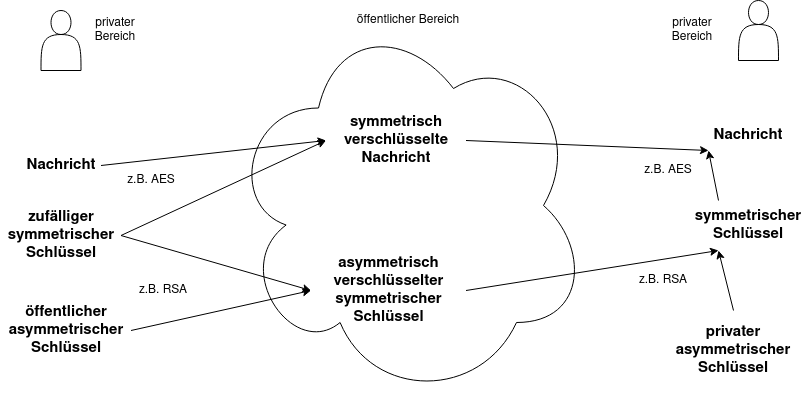
\includegraphics[width=\textwidth]{hybrid.png}
    \caption{Schema zur hybriden Kryptographie.
    Eine Nachricht wird von links nach rechts "uber ein unsicheres Medium (z.B.\@ Internet) verschickt.
    Wie der "offentliche asymmetrische Schl"ussel (sicher) verteilt wird, ist nicht dargestellt.}
    \label{fig:hybrid_crypto}
\end{figure}

Neben Unterschriften "uber Daten sieht OpenPGP auch Unterschriften "uber Schl"us\-sel vor,
die entweder einem Hauptschl"ussel erlauben, Unterschl"ussel an sich zu binden oder
einer Person erlauben, die Genauigkeit einer "`User ID"', also der Zuordnung eines Schl"ussels
zu einer realen Person, zu best"atigen~\cite{rfc4480}.
Letztere erlauben es, ohne direkten (pers"onlichen) Austausch von Schl"usseln mit Personen
verschl"usselt zu kommunizieren, indem man erhaltene Schl"ussel "uber Unterschriften
durch Personen, die man bereits kennt, validiert. \todo{Bild?}

OpenPGP definiert 17 verschiedene "`Packets"',%
\footnote{Die komplette Liste ist entweder mit Erkl"arungen im Standard~\cite{rfc4480}
oder ohne weitere Erl"auterung in \texttt{openpgp/common.py} ab Zeile 200 zu finden.}
die von "offentlichen oder privaten Schl"usseln "uber
"`User IDs"' bis zu verschl"usselten Daten verschiedensten Inhalt haben k"onnen.
Ein OpenPGP-formatierter Datensatz (also z.B.\@ eine verschl"usselte Nachricht, eigene private Schl"ussel,
"offentliche Schl"ussel von Bekannten, usw.\@) besteht aus einer Folge dieser Packets~\cite{rfc4480}.
So w"urde beispielsweise eine an zwei Personen verschl"usselte und unterschriebene Datei im OpenPGP-Format
zwei Packets mit dem asymmetrisch verschl"usselten symmetrischen Schl"ussel und einem Packet mit
verschl"usselten Daten, welches aus Packets f"ur die Datei und die Unterschrift
(sowie ggf.\@ einem weiteren Packet, welches Modifikationen der verschl"usselten Daten erkennbar machen soll)
besteht, enthalten.
Siehe zu diesem Beispiel auch Abbildung~\ref{fig:example_openpgp_format}.

\begin{figure}
    \centering
    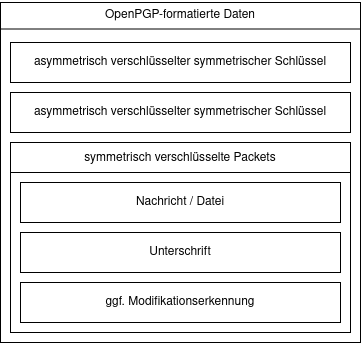
\includegraphics[height=0.3\textheight]{example_openpgp_format.png}
    \caption{Packets in einer an zwei Personen verschl"usselten und unterschriebenen Nachricht.}
    \label{fig:example_openpgp_format}
\end{figure}

\subsection{Meine Implementation}
%Was habe ich implementiert? Auf die hybride Krypto eingehen (AES als Unterpunkt?). Wenn erlaubt/noch Seiten "ubrig, auch auf Datenstrukturen eingehen (die wohl eher Richtung Mathe gehen als Packet-Format lesen usw.)
%Wahrscheinlich auch viel aus dem OpenPGP-Standard zitieren.

Meine OpenPGP-Teilimplementation umfasst:
\begin{itemize}
    \item Einlesen von verschl"usselten Daten (optional mit Modifikationserkennung)
    \item Einlesen von "offentlichen und privaten Schl"usseln (ohne symmetrische Verschl"usselung privater Schl"ussel)
    \item Verifizieren von Unterschriften "uber Daten, User IDs und Unterschl"ussel (nur RSA mit der SHA-Familie)
    \item Erstellen von Unterschriften (nur RSA mit der SHA-Familie "uber Daten)
    \item Verschl"usseln von Daten (nur asymmetrisch mit RSA, symmetrisch mit der AES-Familie, nicht mit Passwort)
\end{itemize}

Intern werden die vielen m"oglichen OpenPGP-Packets in die drei Hauptentit"aten
Schl"ussel, Nachricht (oder Datei) und Unterschrift zusammengefasst,
wobei Unterschriften immer Schl"usseln oder Nachrichten zugeordnet werden.
Aus dieser Darstellung werden dann je nach dem, was gemacht werden soll,
neue Nachrichten, Unterschriften oder verschl"usselte Packets erstellt,
die dann ausgegeben werden.

\todo{Mehr schreiben}

\subsection{Beispiele}
Alle der folgenden Beispiele beginnen mit einer Shell-Zeile, die mit \verb|$| beginnt,
und zeigen danach die jeweiligen Ausgaben.
Im Anhang wird erl"autert, wie sich die genannten Beispiele reproduzieren lassen
(mit anderen Schl"usselfingerabdr"ucken) und wie andere Beispieldateien betrachtet werden k"onnen.

\lstset{
breaklines,
basicstyle=\scriptsize\ttfamily,
language=none,
}

\paragraph{Infos zu geladenen Daten}~
\begin{lstlisting}
$ python3 -m openpgp info
2020-09-20 14:56:46,804 - WARNING(openpgp.signature): unknown signing key f7c5ca02d089077b3536760b42dc1e50d31108cb
Keys:
------------------------------
Key Pair 4e339f0639d483e03fd4dd7b22f24394feb09179
        UID 'Testing Key 1 <testkey-1-openpgp-fa-mathe-sgb@mikitsu.me>'
                GENERIC_UID signature (RSA/SHA256) by b91294876bd058ff9abce9809ad2041a28dc342d, created 2020-08-22 19:21:28, exportable, revocable
                POSITIVE_UID signature (RSA/SHA256) by 4e339f0639d483e03fd4dd7b22f24394feb09179, created 2020-08-22 19:21:27, exportable, revocable
        UID 'Alternative UID <testkey-1-alt-uid-openpgp-fa-mathe-sgb@mikitsu.me>'
                POSITIVE_UID signature (RSA/SHA256) by 4e339f0639d483e03fd4dd7b22f24394feb09179, created 2020-08-22 19:21:28, exportable, revocable
        Key Pair ab81c14d62c5f29ace16d1f61fca78e3f66150ec
                SUBKEY_BIND signature (RSA/SHA256) by 4e339f0639d483e03fd4dd7b22f24394feb09179, created 2020-08-22 19:21:27, exportable, revocable
Public Key b91294876bd058ff9abce9809ad2041a28dc342d
        UID 'Testing Key 2 <testkey-2-openpgp-fa-mathe-sgb@mikitsu.me>'
                GENERIC_UID signature (RSA/SHA256) by 4e339f0639d483e03fd4dd7b22f24394feb09179, created 2020-08-22 19:21:28, exportable, revocable
                POSITIVE_UID signature (RSA/SHA256) by b91294876bd058ff9abce9809ad2041a28dc342d, created 2020-08-22 19:21:27, exportable, revocable
        Public Key 0bca1709a0c297a5fa8e8e6850587fe80adf2136
                SUBKEY_BIND signature (RSA/SHA256) by b91294876bd058ff9abce9809ad2041a28dc342d, created 2020-08-22 19:21:27, exportable, revocable
\end{lstlisting}

Es werden alle User IDs angezeigt, man sieht, dass zum ersten Schl"ussel auch der private Teil verf"ugbar ist (\texttt{Key Pair}).
Die Unterschriften bez"uglich der Verifizierung (\texttt{POSITIVE\_UID}/\texttt{GENERIC\_UID})
und der Unterschl"usselbindung (\texttt{SUBKEY\_BIND}) werden angezeigt.
Eine Unterschrift stammt von einem unbekannten Schl"ussel und wird daher nicht angezeigt.
Im Folgenden wird diese Warnung weggelassen.

\paragraph{Einlesen von Nachrichten}~\\
Unterschriebene Nachrichten werden validiert.
Angezeigt werden Unterschriften und Nachrichtvorschau.
\begin{lstlisting}
$ python3 -m openpgp --load data/text-message info
Keys:
------------------------------
[entfernt]

Messages:
------------------------------
'Hello there.\nThis is a ...Windows and Mac.\nBye!\n'
        file "", 2020-08-22 19:21:28
        TEXT signature (RSA/SHA512) by 0bca1709a0c297a5fa8e8e6850587fe80adf2136, created 2020-08-22 19:21:28, exportable, revocable
\end{lstlisting}
Zum Speichern von Nachrichten werden diesen zum STDOUT geschrieben.
Durch Umleitung kann man sie in Dateien speichern.
\begin{lstlisting}
$ python3 -m openpgp --load data/text-message save-message
Hello there.
This is a test text.
Using text mode should handle line endings
and make me be five (plus a trailing newline) lines long even on Windows and Mac.
Bye!
\end{lstlisting}

\paragraph{Erstellen von Nachrichten}
Um eine Datei zu unterschrieben und verschl"usseln, muss man:
\begin{enumerate}
    \item Die Datei (hier \texttt{/bin/true}) ins OpenPGP-Format konvertieren
    \item Die Datei mit dem/den eigenen privaten Schl"ussel(n) unterschrieben
    \item Die Datei verschl"usseln, wobei die eigentliche Datei symmetrisch
        und nur der symmetrische Schl"ussel asymmetrisch verschl"usselt wird.
        Es ist sinnvoll, an dieser Stelle auch an sich selbst zu verschl"usseln.
\end{enumerate}
Hier wird auch das Entschl"usseln und der Vergleich mit der Originaldatei gezeigt.
\begin{lstlisting}
$ python3 -m openpgp pgpify /bin/true \
  | python3 -m openpgp -l- sign 'Key 1' \
  | python3 -m openpgp -l- sign ab81c14d62c5f29ace16d1f61fca78e3f66150ec \
  | python3 -m openpgp -l- encrypt --recipient 'Key 2' --recipient alt-uid --symm-algo AES128 > /tmp/encrypted-true
$ python3 -m openpgp --load /tmp/encrypted-true info
Keys:
------------------------------
Key Pair 4e339f0639d483e03fd4dd7b22f24394feb09179
        [UIDs entfernt]
        Key Pair ab81c14d62c5f29ace16d1f61fca78e3f66150ec
                [Unterschrift entfernt]
Public Key b91294876bd058ff9abce9809ad2041a28dc342d
        [UID entfernt]
        Public Key 0bca1709a0c297a5fa8e8e6850587fe80adf2136
                [Unterschrift entfernt]

Messages:
------------------------------
<binary data>
        file "/bin/true", 2020-09-24 16:35:21
        BINARY signature (RSA/SHA256) by 4e339f0639d483e03fd4dd7b22f24394feb09179, created 2020-09-24 16:35:21, exportable, revocable
        BINARY signature (RSA/SHA256) by ab81c14d62c5f29ace16d1f61fca78e3f66150ec, created 2020-09-24 16:35:21, exportable, revocable
$ python3 -m openpgp --load /tmp/encrypted-true save-message >/tmp/decrypted-true
$ sha256sum /bin/true /tmp/decrypted-true
65fd744686e1c8ad156c57637e3cb3c76f003cf075a67eed287667ab969503a5  /bin/true
65fd744686e1c8ad156c57637e3cb3c76f003cf075a67eed287667ab969503a5  /tmp/decrypted-true
\end{lstlisting}

\paragraph{Was nicht funktioniert}~\\
Ohne privaten Schl"ussel ist offensichtlich sowohl Unterschreiben als auch Entschl"usseln unm"oglich:
\begin{lstlisting}
$ python3 -m openpgp pgpify /bin/true | python -m openpgp -l- encrypt --recipient 'Key 2' | python -m openpgp -l- info
2020-09-24 16:49:18,713 - ERROR(openpgp.parse): No session key. Encrypted for: ['9ad2041a28dc342d']
Keys:
------------------------------
Key Pair 4e339f0639d483e03fd4dd7b22f24394feb09179
        [UIDs entfernt]
        Key Pair ab81c14d62c5f29ace16d1f61fca78e3f66150ec
                [Unterschrift entfernt]
Public Key b91294876bd058ff9abce9809ad2041a28dc342d
        [UID entfernt]
        Public Key 0bca1709a0c297a5fa8e8e6850587fe80adf2136
                [Unterschrift entfernt]
$ python3 -m openpgp pgpify /bin/true | python -m openpgp -l- sign 'Key 2'
No such key:  Key 2
\end{lstlisting}

\section{Ausleitung}
Facharbeitshinweise:
\begin{quote}
Der Schluss sollte die Fragestellung aus der Einleitung aufgreifen und die wichtigsten Untersuchungsergebnisse zusammenfassen. Er kann den Untersuchungsgegenstand in größere Zusammenhänge einordnen und einen Ausblick auf künftige Entwicklungen enthalten. Auch kann hier das methodische Vorgehen kritisch reflektiert werden.
\end{quote}

RSA fu"st, wie in dieser Arbeit deutlich gemacht, auf zwei Grundlagen:
die der modularen Arithmetik, besonders in Kombination mit Exponentiation
und die der Primzahlen.

Modulare Arithmetik spielt auch in anderen asmmetrischen Kryptosystemen,
wie etwa dem Diffie-Hellmen key exchange oder ElGamal, eine gro"se Rolle.
Entsprechend ist auch die praktische Verschnellerung odularer Exponentiation
weitlaufend untersucht.
In dieser Arbeit ist nur eine simple Grundlage n"aher besprochen worden,
jedoch sind Leser eingeladen, auch "uber andere bzw.\@ verbesserte Ans"atze
in Kapitel 14.6 der Quelle~\cite{hac} zu lesen.

Primzahlen, von ihrer mathematischen Natur aus eines der abstraktesten Themen,
sind durch asymmetrische Kryptographie wichtig in der praktischen Anwendung geworden.
Insgesamt hat die Zahlentheorie durch asymmetrische Kryptographie enorm an praktischer Bedeutung gewonnen.

Obwohl derzeit auf elliptischen Kurven (auch eine sehr abstrakte methematische Grundlage)
basierende asymmetrische Kryptographie st"arker verwendet wird,
ist absehbar, dass RSA f"ur die breiten Bev"olkerungsmassen als Bestandteil
der TLS-Rootzertifikate in Webbrowsern noch Jahre und in speziellen Anwendungen m"oglicherweise
noch Jahrzehnte relevant bleiben wird.

W"ahrend OpenPGP selbst f"ur die meisten Menschen nur indirekt relevant ist,
z.B.\@ "uber GPG-unterschriebene git-Tags neuer Linux-Versionen, welche die Grundlage f"ur Android bilden,
sind die allgemeinen Konzepte beispielsweise bez"uglich hybrider Kryptographie allgemein
auf viele praktische Anwendungen direkt "ubertragbar.

\appendix

\addcontentsline{toc}{section}{Literatur}
\begin{thebibliography}{9}
\bibitem{rsa}
1. Rivest, R. L., 2. Shamir, A. und 3. Adleman, L.:
A method for obtaining digital signatures and public-key cryptosystems.
In: Communications of the ACM, Band 21 / Ausgabe 2 Februar 1978, S. 120 - 126

\bibitem{hac}
1. Menezes, Alfred J., 2. van Oorschot, Paul C und 3. Vanstone, Scott A.:
Handbook of applied cryptography.
London: CRC Press 2001

\bibitem{rfc4480}
1. Callas, J., 2. Donnerhacke, L., 3. Finney,~H., 4. Shaw,~D. und 5. Thayer,~R.:
OpenPGP Message Format. RFC 4880. November 2007

\bibitem{euler41}
Euler, Leonhard: Theorematum quorundam ad numeros primos spectantium demonstratio.
1741. Abgerufen "uber: Euler Archive - All Works by Enestr"om Number. 54.
https://scholarlycommons.pacific.edu/euler-works/54

\bibitem{euler63}
Euler, Leonhard: Theoremata arithmetica nova methodo demonstrata.
1763. Abgerufen "uber: Euler Archive - All Works by Enestr"om Number. 271.
https://scholarlycommons.pacific.edu/euler-works/271

\bibitem{sinews}
Robinson, Sara: Still Guarding Secrets after Years of Attacks, RSA Earns Accoladesfor its Founders
In: SIAM News, Ausgabe 5 Juni 2003.
Abgerufen "uber: https://archive.siam.org/pdf/news/326.pdf

\bibitem{singh}
Singh, Simon: The Code Book. New York: Doubleday 1999

\bibitem{taocp2}
Knuth, Donald Erwin: The Art of Computer Programming / Volume 2: Seminumerical Alogrithms.
Reading: Addison-Wesley 1997

\piicitations
\end{thebibliography}


\section{kompletter Quellcode}
\todo{sind ca. 30 Seiten}
\lstset{language=Python}
%\lstinputlisting{../openpgp/__main__.py}
%\lstinputlisting{../openpgp/rsa.py}
%\lstinputlisting{../openpgp/common.py}
%\lstinputlisting{../openpgp/parse.py}
%\lstinputlisting{../openpgp/signature.py}
%\lstinputlisting{../openpgp/create.py}
%\lstinputlisting{../openpgp/display.py}
%\lstinputlisting{../openpgp/helpers.py}
%\lstinputlisting{../openpgp/aes_ll2.py}
%\lstinputlisting{../openpgp/openpgp_cfb.py}

\section{Beispieldateien}

\todo{Hochladen}

\section{Internetquellen}

\paragraph{\cite{euler41}}
\includegraphics[width=\textwidth]{euler-54.pdf}
\paragraph{\cite{euler63}}
\includegraphics[width=\textwidth]{euler-271.pdf}
\paragraph{\cite{sinews}}
\includegraphics[width=\textwidth]{sinews.pdf}

\section{Selbst"andigkeitserkl"arung}
Ich habe die vorliegende Facharbeit selbständig angefertigt und keine anderen als die angegebenen Hilfsmittel benutzt.
Alle "ubernommenen Textteile sind als Zitate gekennzeichnet und mit genauer Quellenangabe belegt. \\~\\
\rule{0.3\textwidth}{1pt}~\\
\piisignature
\end{document}
